%%%%%%%%%%%%%%%%%%%%%%%%%%%%%%%%%%%%%%%%%
% Beamer Presentation
% LaTeX Template
% Version 1.0 (10/11/12)
%
% This template has been downloaded from:
% http://www.LaTeXTemplates.com
%
% License:
% CC BY-NC-SA 3.0 (http://creativecommons.org/licenses/by-nc-sa/3.0/)
%
%%%%%%%%%%%%%%%%%%%%%%%%%%%%%%%%%%%%%%%%%

%----------------------------------------------------------------------------------------
%	PACKAGES AND THEMES
%----------------------------------------------------------------------------------------

\documentclass{beamer}

\mode<presentation> {

% The Beamer class comes with a number of default slide themes
% which change the colors and layouts of slides. Below this is a list
% of all the themes, uncomment each in turn to see what they look like.

%\usetheme{default}
%\usetheme{AnnArbor}
%\usetheme{Antibes}
%\usetheme{Bergen}
%\usetheme{Berkeley}
%\usetheme{Berlin}
%\usetheme{Boadilla}
%\usetheme{CambridgeUS}
%\usetheme{Copenhagen}
%\usetheme{Darmstadt}
%\usetheme{Dresden}
%\usetheme{Frankfurt}
%\usetheme{Goettingen}
%\usetheme{Hannover}
%\usetheme{Ilmenau}
%\usetheme{JuanLesPins}
%\usetheme{Luebeck}
\usetheme{Madrid}
%\usetheme{Malmoe}
%\usetheme{Marburg}
%\usetheme{Montpellier}
%\usetheme{PaloAlto}
%\usetheme{Pittsburgh}
%\usetheme{Rochester}
%\usetheme{Singapore}
%\usetheme{Szeged}
%\usetheme{Warsaw}

% As well as themes, the Beamer class has a number of color themes
% for any slide theme. Uncomment each of these in turn to see how it
% changes the colors of your current slide theme.

%\usecolortheme{albatross}
%\usecolortheme{beaver}
%\usecolortheme{beetle}
%\usecolortheme{crane}
%\usecolortheme{dolphin}
%\usecolortheme{dove}
%\usecolortheme{fly}
%\usecolortheme{lily}
%\usecolortheme{orchid}
%\usecolortheme{rose}
%\usecolortheme{seagull}
%\usecolortheme{seahorse}
%\usecolortheme{whale}
%\usecolortheme{wolverine}

%\setbeamertemplate{footline} % To remove the footer line in all slides uncomment this line
%\setbeamertemplate{footline}[page number] % To replace the footer line in all slides with a simple slide count uncomment this line

%\setbeamertemplate{navigation symbols}{} % To remove the navigation symbols from the bottom of all slides uncomment this line
}

\usepackage{graphicx} % Allows including images
\usepackage{booktabs} % Allows the use of \toprule, \midrule and \bottomrule in tables
\usepackage{multirow}
\usepackage{adjustbox}
\usepackage{array}
\usepackage{tikz}
\usepackage{soul}
\usepackage{pdfpages}
\usetikzlibrary{shapes.geometric, arrows, positioning, fit}
\usepackage[latin1]{inputenc}
\newcommand{\xmark}{\textcolor{red}{\text{\sffamily X}}}
\newcommand{\cmark}{\textcolor{green}{\checkmark}}
\newcommand{\tr}{\text{tr}}
\newcommand{\E}{\textbf{E}}
\newcommand{\diag}{\text{diag}}
\newcommand{\argmax}{\text{argmax}}
\newcommand{\argmin}{\text{argmin}}
\newcommand{\Cov}{\text{Cov}}
\newcommand{\Var}{\text{Var}}
\newcommand{\Vol}{\text{Vol}}
\newcommand{\bx}{\boldsymbol{x}}
\newcommand{\by}{\boldsymbol{y}}
\newcommand{\bX}{\boldsymbol{X}}
\newcommand{\bY}{\boldsymbol{Y}}
\sethlcolor{gray}
\makeatletter
\newcommand\SoulColor{%
  \let\set@color\beamerorig@set@color
  \let\reset@color\beamerorig@reset@color}
\makeatother
\definecolor{color1}{RGB}{128,13,13}
\definecolor{color2}{RGB}{70,128,13}
\definecolor{color3}{RGB}{13,128,128}
\definecolor{color4}{RGB}{70,13,128}

%tikz stufff


%----------------------------------------------------------------------------------------
%	TITLE PAGE
%----------------------------------------------------------------------------------------


\title[Inference through learning]{What does classification tell us about the brain? Statistical inference through machine learning}

\author{Charles Zheng} % Your name
\institute[Stanford] % Your institution as it will appear on the bottom of every slide, may be shorthand to save space
{Stanford University}
\date{\today} % Date, can be changed to a custom date

\begin{document}

\begin{frame}
\titlepage % Print the title page as the first slide
(Joint work with Yuval Benjamini.)
\end{frame}

\section{Introduction}

\begin{frame}
\frametitle{Studying the neural code}
\begin{center}
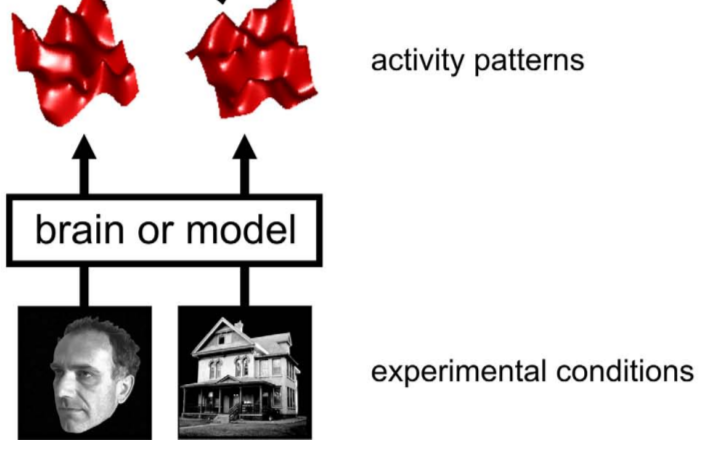
\includegraphics[scale = 0.3]{k08_step1.png}
\end{center}
Present the subject with visual stimuli, pictures of faces and houses.
Record the subject's brain activity in the fMRI scanner.
\end{frame}




\begin{frame}
\frametitle{Studying the neural code: data}
\begin{center}
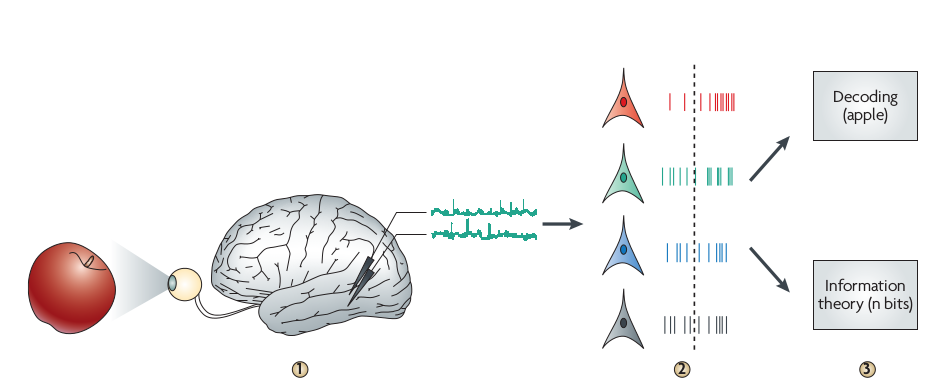
\includegraphics[scale = 0.2]{quiroga.png}
\end{center}
\begin{itemize}
\item  Let $\mathcal{X}$ define a class of stimuli (faces, objects, sounds.)
\item Stimulus $\bX = (X_1,\hdots, X_p)$, where $X_i$ are features (e.g. pixels.)
\item Present $\bX$ to the subject, record the subject's brain activity using EEG, MEG, fMRI, or calcium imaging.
\item Recorded response $\bY = (Y_1,\hdots, Y_q)$, where $Y_i$ are single-cell responses, or recorded activities in different brain region. 
\end{itemize}
\tiny{Image credits: Quiroga et al. (2009).}
\end{frame}

\begin{frame}
\frametitle{Experimental design}
\begin{itemize}
\item How to make inferences about the population of stimuli in
  $\mathcal{X}$ using finitely many examples?
\item \emph{Randomization.}  Select $\bX^{(1)},\hdots,
  \bX^{(K)}$ randomly from some distribution $p(\bx)$ (e.g. an image
  database).  Record $r$ responses from each stimulus.
\end{itemize}
\begin{center}
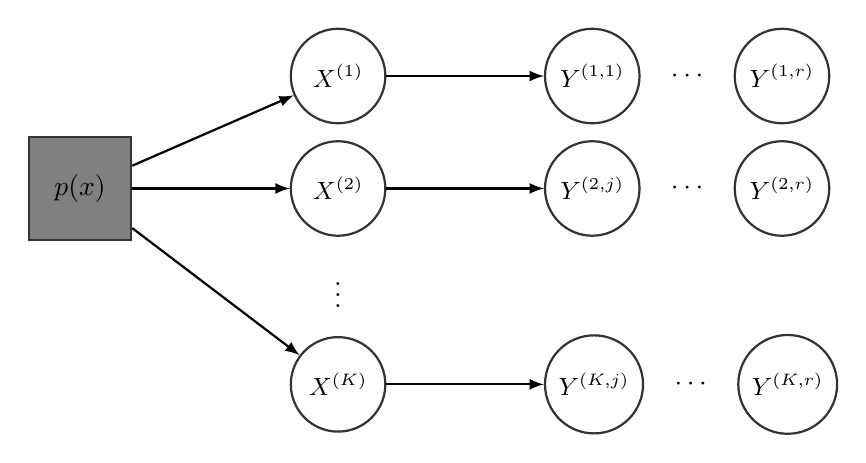
\begin{tikzpicture}[node distance = 2mm and 20mm]
\tikzstyle{main} = [circle, minimum size = 12mm, thick, draw = black!80]
\tikzstyle{main0} = [circle, minimum size = 2mm, thick, draw = white!100]
\tikzstyle{param} = [rectangle, minimum size = 13mm, thick, draw = black!80]
\tikzstyle{connect} = [-latex, thick]
\tikzstyle{box} = [rectangle, draw = black!100]
  \node[param, fill = black!50] (px) {$p(\bx)$};
  \node[main, right=of px] (x2) {\small{$\bX^{(2)}$}};
  \node[main, above=of x2] (x1) {\small{$\bX^{(1)}$}};
  \node[main0, below=of x2] (xdots) {$\vdots$};
  \node[main, below=of xdots] (x3) {\small{$\bX^{(K)}$}};
  \node[main, right=of x1] (y11) {\small{$\bY^{(1,1)}$}};
  \node[main, right=of x2] (y21) {\small{$\bY^{(2,j)}$}};
  \node[main, right=of x3] (y31) {\small{$\bY^{(K,j)}$}};
\begin{scope}[node distance = 3mm and 2mm]
  \node[main0, right=of y11] (y12) {$\cdots$};
  \node[main0, right=of y21] (y22) {$\cdots$};
  \node[main0, right=of y31] (y32) {$\cdots$};
  \node[main, right=of y12] (y13) {\small{$\bY^{(1,r)}$}};
  \node[main, right=of y22] (y23) {\small{$\bY^{(2,r)}$}};
  \node[main, right=of y32] (y33) {\small{$\bY^{(K,r)}$}};
\end{scope}
\path (px) edge [connect] (x1) (px) edge [connect] (x2) (px) edge [connect] (x3)
      (x1) edge [connect] (y11) (x2) edge [connect] (y21) (x3) edge [connect] (y31);
\end{tikzpicture}
\end{center}
\end{frame}

\begin{frame}
\frametitle{Analyzing the data using machine learning}
\begin{itemize}
\item Now we have data consisting of (stimulus, reponse) pairs.
\item Can we classify the response using the stimulus?  What is the confusion matrix?
\end{itemize}
\end{frame}

\begin{frame}
\frametitle{Gaussian example}
To help think about these problems, consider a concrete example:
\begin{itemize}
\item Let $\bX \sim N(0, I_d)$ and 
$\bY|\bX \sim N(\bX,\sigma^2 I_d)$.
\item We draw stimuli $\bx^{(1)}, \hdots, \bx^{(K)} \sim N(0, I_d)$ i.i.d.
\item For each stimulus $\bx^{(i)}$, we draw observations $\by^{(i, j)} = \bx^{(i)} + \epsilon^{(i, j)}$, where $\epsilon^{(i, j)} \sim N(0, \sigma^2 I_d)$.
\end{itemize}
\begin{center}
\begin{tabular}{ccc}
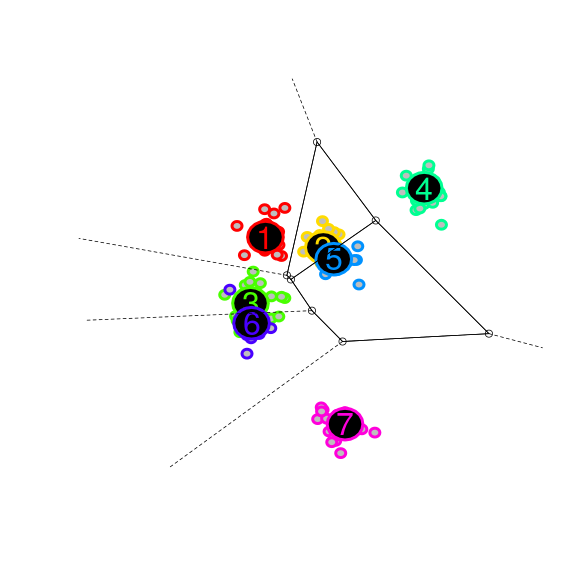
\includegraphics[scale = 0.2, clip = true, trim = 0.6in 0.2in 0.6in 0.2in]{../info_theory_paper/gaussian_figure1a.png} &
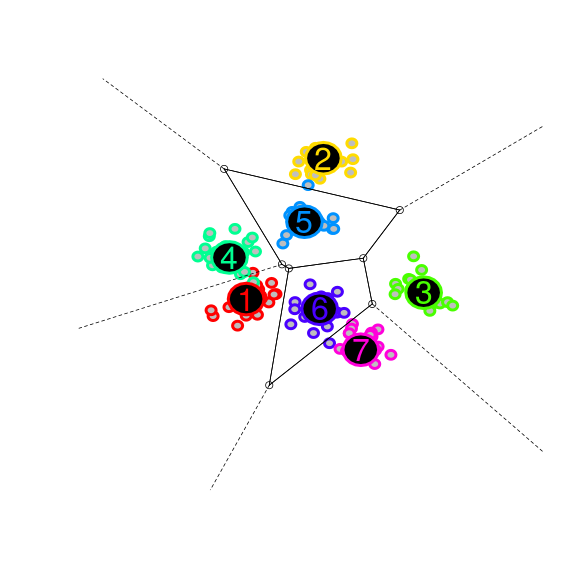
\includegraphics[scale = 0.2, clip = true, trim = 0.6in 0.2in 0.6in 0.2in]{../info_theory_paper/gaussian_figure1b.png} &
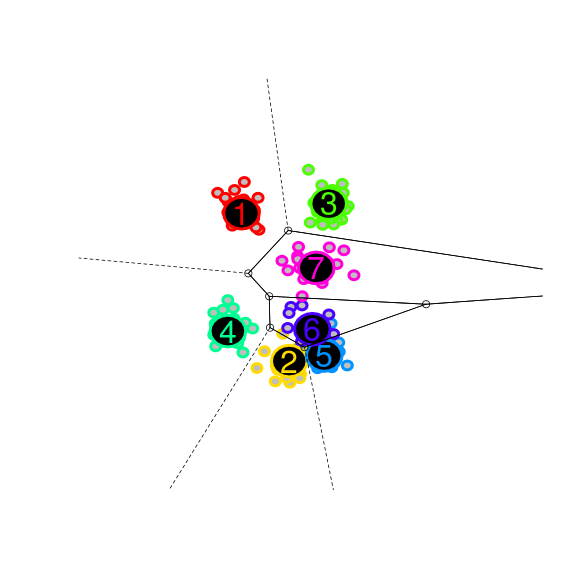
\includegraphics[scale = 0.2, clip = true, trim = 0.6in 0.2in 0.6in 0.2in]{../info_theory_paper/gaussian_figure1c.png}
\end{tabular}
\end{center}
\end{frame}


\begin{frame}
\frametitle{Motivation for my research}
Ultimately, the goal of these experiments is to understand the
  dependence between $X$ (stimulus) and $Y$ (the brain response). 

Possible goals for statistical methodology (which currently don't exist):
\begin{enumerate}
\item What can be inferred from the classification accuracy?
\item Can we predict what the result (classification accuracy) would be in a similar (but possibly larger or smaller) experiment?
\item Can we \emph{summarize} the total information content contained
  in $Y$ about $X$?
\item Can we \emph{decompose} the total information contained in $Y$ about $X$?  (Something like a nonlinear ANOVA decomposition?)
\end{enumerate}
\end{frame}

\begin{frame}
\frametitle{Motivation 1: What can be inferred from the classification accuracy?}
\begin{itemize}
\item The achieved classification accuracy is an estimate of \emph{generalization accuracy}...
\item which in turn lower bounds on the generalization error of the best classifier, the \emph{Bayes accuracy}.
\item But the Bayes accuracy varies depending on the stimuli set $\bX^{(1)},\hdots, \bX^{(K)}$!
\[
\text{BA}(X_1,...,X_k)
\]
\end{itemize}
Define \emph{average Bayes accuracy} as the expected Bayes accuracy
\[
\text{ABA}_k = \E[\text{BA}(X_1,...,X_k)]
\]
where expectation is taken over sampling $X_1,..,X_k$ from $p(x)$.
\end{frame}

\begin{frame}
\frametitle{Average Bayes accuracy}
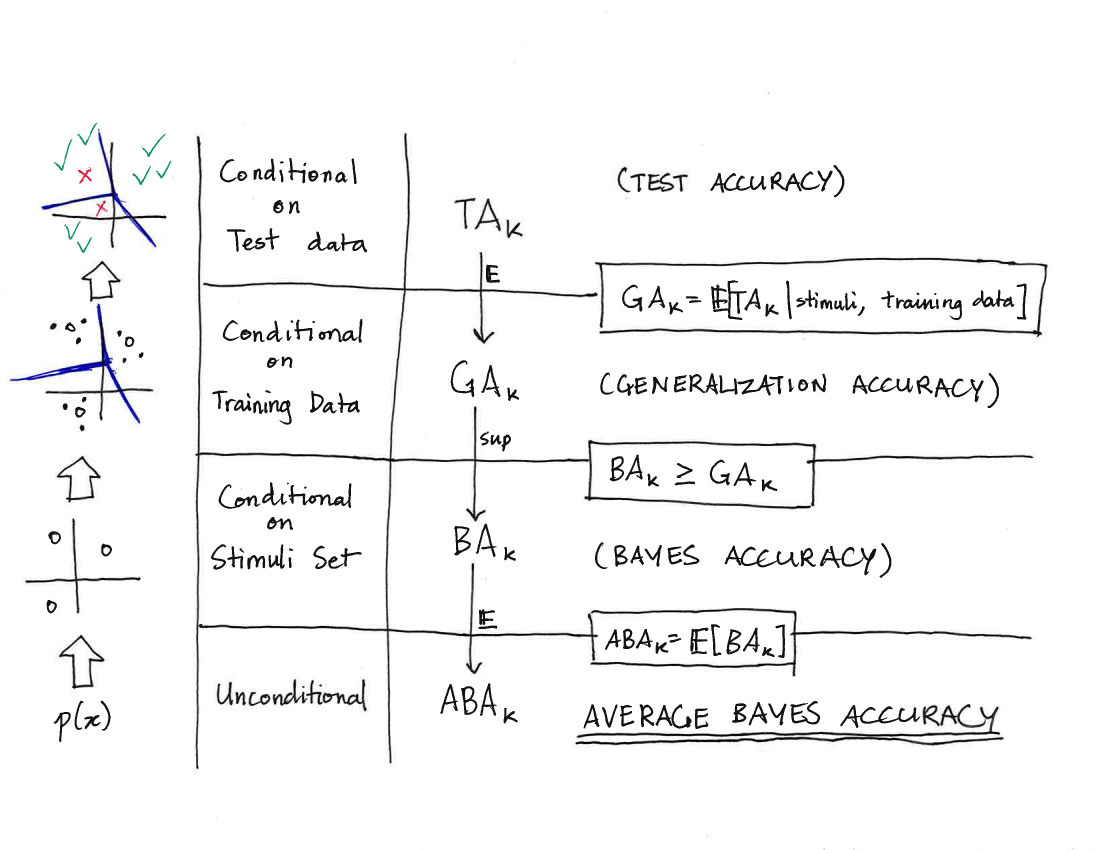
\includegraphics[scale = 0.45, clip = true, trim = 0in 1in 0.5in 1in]{ta_to_aba.png}
\end{frame}

\begin{frame}
\frametitle{Inferring average Bayes accuracy}
\begin{itemize}
\item We cannot observe either $\text{ABA}_k$, or even $\text{BA}_k$.
\item However, we can obtain a \emph{lower confidence bound} for $\text{BA}_k$, since the generalization accuracy is an \emph{underestimate} of $\text{BA}_k$
\item But we actually want a lower confidence bound for $\text{ABA}_k$!
\end{itemize}
\end{frame}

\begin{frame}
\frametitle{Concentration of Bayes accuracy}
Recall that
\[
\text{ABA}_k = \textbf{E}[\text{BA}_k]
\]

Converting a LCB for $\text{BA}_k$ to an LCB on $\text{ABA}_k$ boils down to the following problem:
\vspace{0.2in}

\emph{What is the variability of }$\text{BA}_k$?
\vspace{0.2in}

We will discuss this later in the talk!
\end{frame}


\begin{frame}
\frametitle{Motivation 2: Generalizing to similar designs}
Define $\text{ABA}_k$ as the average Bayes accuracy for $k$ classes.

Can we predict $\text{ABA}_{100}$ given data from 30 classes?  See Z., Achanta and Benjamini (2016).
\begin{figure}
\centering
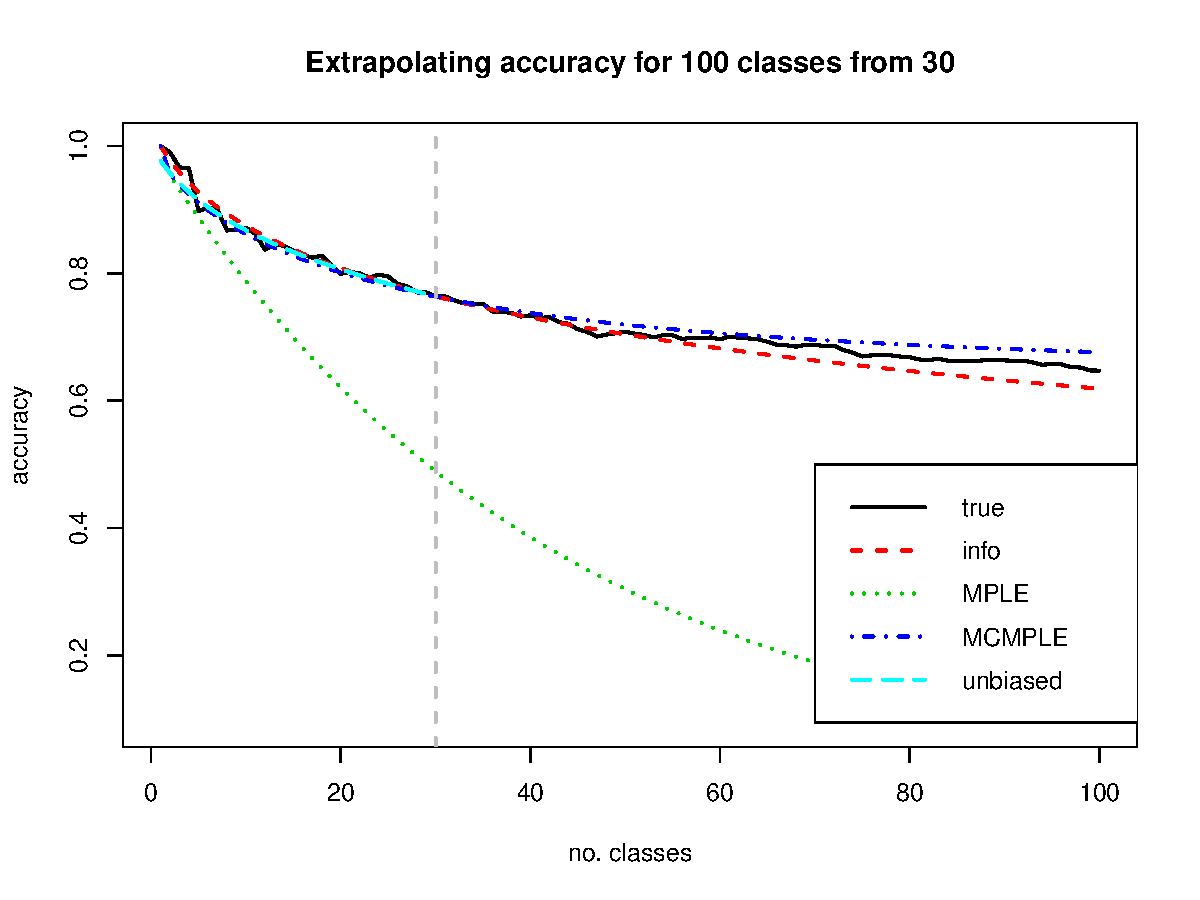
\includegraphics[scale = 0.4]{../info_theory_paper/cifar_example.pdf}
\end{figure}
\end{frame}

\begin{frame}
\frametitle{Motivation 3 and 4: Quantifying and decomposing information}
\emph{Can we \emph{summarize} the total information content contained
  in $Y$ about $X$?

Can we \emph{decompose} the total information contained in $Y$ about $X$?}
\vspace{0.5in}


The answer is yes, and the solution was provided by Claude Shannon.
\emph{Mutual information} measures the information contained in $Y$
about $X$ (or vice versa) in a nonlinear way.
\end{frame}

\begin{frame}
\frametitle{Mutual information}
\end{frame}

\section{Variability of Bayes accuracy}

\begin{frame}
\sectionpage
\end{frame}

\begin{frame}
\frametitle{Definitions}
\begin{itemize}
\item Suppose $(X, Y)$ have a joint density $p(x, y)$,
\item The Bayes accuracy is a function of the stimuli set $x_1,...,x_k$,
\[
\text{BA}(x_1,...,x_k)
\]
\item Draw $Z \sim \{1,...,k\}$, and draw $Y \sim p(y|x_z)$.
\item Let $f$ (the \emph{classifier}) that associates a label $\{1,...,k\}$ to each possible value of $y$:
\[
f: \mathcal{Y} \to \{1,...,k\}
\]
\item Define
\[
\text{BA}(x_1,...,x_k) = \sup_f \Pr[f(Y) = Z| x_1,...,x_k]
\]
where the probability is over the joint distribution $(Y, Z)$ defined above.
Notice we condition on the particular stimuli set $x_1,...,x_k$.
\end{itemize}
\end{frame}


\begin{frame}
\frametitle{An identity}
\begin{itemize}
\item It is a well-known result from Bayesian inference that the optimal classifier $f$ is defined as
\[
f(y) = \text{argmax}_{i=1}^k p(y|x_i),
\]
since the prior class probabilities are uniform.
\item Therefore,
\begin{align*}
\text{BA}(x_1,...,x_k) &= \Pr[\text{argmax}_{i=1}^k p(y|x_i) = Z| x_1,...,x_k] 
\\&= \frac{1}{k}\int \max_{i=1}^k p(y|x_i) dy.
\end{align*}
\end{itemize}
\end{frame}

\begin{frame}
\frametitle{Intuition behind identity}
\begin{columns}
\begin{column}{0.5\textwidth}
\begin{center}
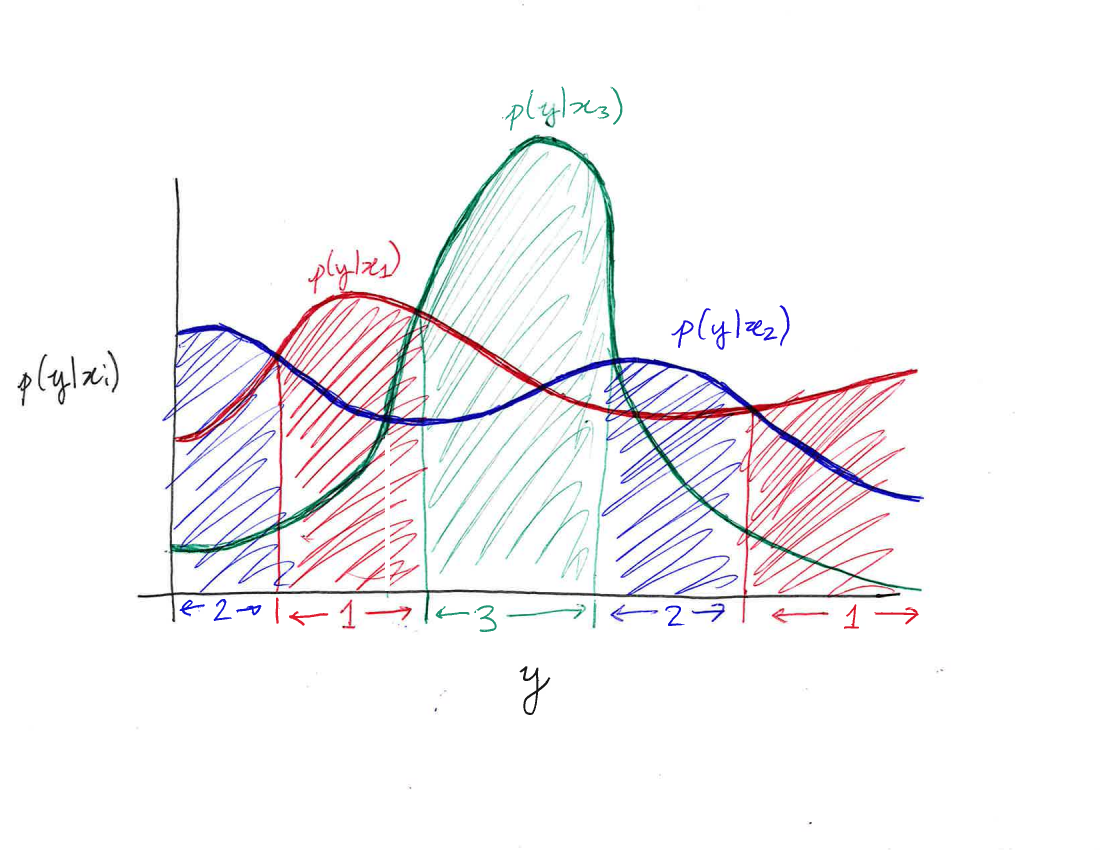
\includegraphics[scale = 0.35, clip = true, trim = 1.2in 1.3in 0in 1in]{var_ba.png}
\end{center}   
\end{column}
\begin{column}{0.5\textwidth}  %%<--- here
\begin{align*}
\text{BA}&(x_1,x_2,x_3) \\&= \sum_i \Pr[x_i]\Pr_{Y \sim p(y|x_i)}[Y \in \text{zone }i]
\\&= \sum_i \frac{1}{k} \text{Area under curve $i$ in zone $i$}
\\&\ \ \ = \frac{1}{k} \text{Area under } \max_{i=1}^k p(y|x_i)
\end{align*}
\end{column}
\end{columns}
\end{frame}

\begin{frame}
\frametitle{Efron-Stein lemma}
\begin{itemize}
\item We have
\[
\text{ABA}_k = \E[\text{BA}(X_1,...,X_k)]
\]
where the expectation is over the independent sampling of $X_1,...,X_k$ from $p(x)$.
\item According to the Efron-Stein lemma,
\[
\text{Var}[\text{BA}(X_1,...,X_k)] \leq \sum_{i=1}^k \E[\text{Var}[\text{BA}|X_1,...,X_{i-1}, X_{i+1}, ..., X_k]].
\]
which is the same as
\[
\text{Var}[\text{BA}(X_1,...,X_k)] \leq k \E[\text{Var}[\text{BA}|X_1,...,X_{k-1}]].
\]
\item The term $\text{Var}[\text{BA}|X_1,...,X_{k-1}]$ is the variance of $\text{BA}(X_1,...,X_k)$
conditional on fixing the first $k-1$ curves $p(y|x_1),...,p(y|x_{k-1})$ and allowing the final curve $p(y|X_k)$ to vary randomly.
\end{itemize}
\end{frame}

\begin{frame}
\frametitle{Efron-Stein lemma}
\begin{itemize}
\item 
\[
\text{Var}[\text{BA}(X_1,...,X_k)] \leq k \E[\text{Var}[BA|X_1,...,X_{k-1}]].
\]
\item Note the following trivial results
\[
-p(y|x_k) + \max_{i=1}^k p(y|x_i)\leq \max_{i=1}^{k-1} p(y|x_i) \leq \max_{i=1}^k p(y|x_i)
\]
\item This implies
\[
\text{BA}(X_1,...,X_k) - \frac{1}{k} \leq \frac{k-1}{k}\text{BA}(X_1,...,X_{k-1}) \leq \text{BA}(X_1,...,X_k).
\]
i.e. conditional on $(X_1,...,X_{k-1})$, $\text{BA}_k$ is supported on an interval of size $1/k$.
\item Therefore,
\[
\text{Var}[\text{BA}|X_1,...,X_{k-1}] \leq \frac{1}{4k^2}
\]
since $\frac{1}{4c^2}$ is the maximal variance for any r.v. with support of length $c$.
\end{itemize}
\end{frame}

\begin{frame}
\frametitle{Variance bound}
Therefore, Efron-Stein bound gives
\[
\text{sd}[\text{BA}_k] \leq \frac{1}{2\sqrt{k}}
\]
Compare this with empirical results (searching for worst-case distributions):
\begin{tabular}{c||c|c|c|c|c|c|c}
k & 2 & 3 & 4 & 5 & 6 & 7 & 8\\\hline
$\frac{1}{2\sqrt{k}}$ & 0.353 & 0.289 & 0.250 & 0.223 & 0.204 & 0.189 & 0.177\\\hline
Worst-case sd & 0.25 & 0.194 & 0.167 & 0.150 & 0.136 & 0.126 & 0.118
\end{tabular}
\end{frame}

\begin{frame}
\frametitle{Improving the variance bound?}
\begin{itemize}
\item All of the worst-case distributions found so far have the
  following simple form:
\[
\mathcal{Y} = \mathcal{X} = \{1,...,d\} \text{ for some } d
\]
\[
p(y|x) = \frac{1}{d}I\{x = y\}
\]
Can we prove this rigorously?
\item Recalling that
\[
\text{BA}(X_1,...,X_k) - \frac{1}{k} \leq \frac{k-1}{k}\text{BA}(X_1,...,X_{k-1}) \leq \text{BA}(X_1,...,X_k).
\]
it is worth noting that distributions of this type actually
concentrate on the two endpoints of the bound, thus in some sense
``maximizing'' the variance.
%\item Distributions of this type actually maximize the variance
%\[\text{Var}[\text{BA}|X_1,...,X_{k-1}]\]
%given a constraint on $\E[BA|X_1,...,X_{k-1}]$,
%since 
%\[
%\text{BA}(X_1,...,X_k) = \begin{cases}
%\frac{k-1}{k}\text{BA}(X_1,..,X_{k-1}) & \text{ if }X_k \in \{X_1,..,X_{k-1}\}\\
%\frac{k-1}{k}\text{BA}(X_1,..,X_{k-1}) + \frac{1}{k} & \text{ otherwise}
%\end{cases}
%\]
\end{itemize}
\end{frame}

\section{Inferring mutual information from classification accuracy}

\begin{frame}
\sectionpage
\end{frame}

\begin{frame}
\frametitle{Outline}
\begin{itemize}
\item We observe $(X, Y)$ pairs from the random-stimulus repeated-sampling design.
\item Goal is to infer $I(X; Y)$, also written $\text{I}[p(x, y)]$.
\end{itemize}
\end{frame}

\begin{frame}
\frametitle{Outline}
\begin{columns}
\begin{column}{0.5\textwidth}
\begin{itemize}
\item Step 1: Apply machine learning to obtain \emph{test accuracy} $\text{TA}_k$
\item Step 2: Infer $\text{ABA}_k$ from $\text{TA}_k$
\item Step 3: Obtain a lower bound on $I(X; Y)$ from $\text{ABA}_k$!
\end{itemize}
\end{column}
\begin{column}{0.5\textwidth}
\begin{center}
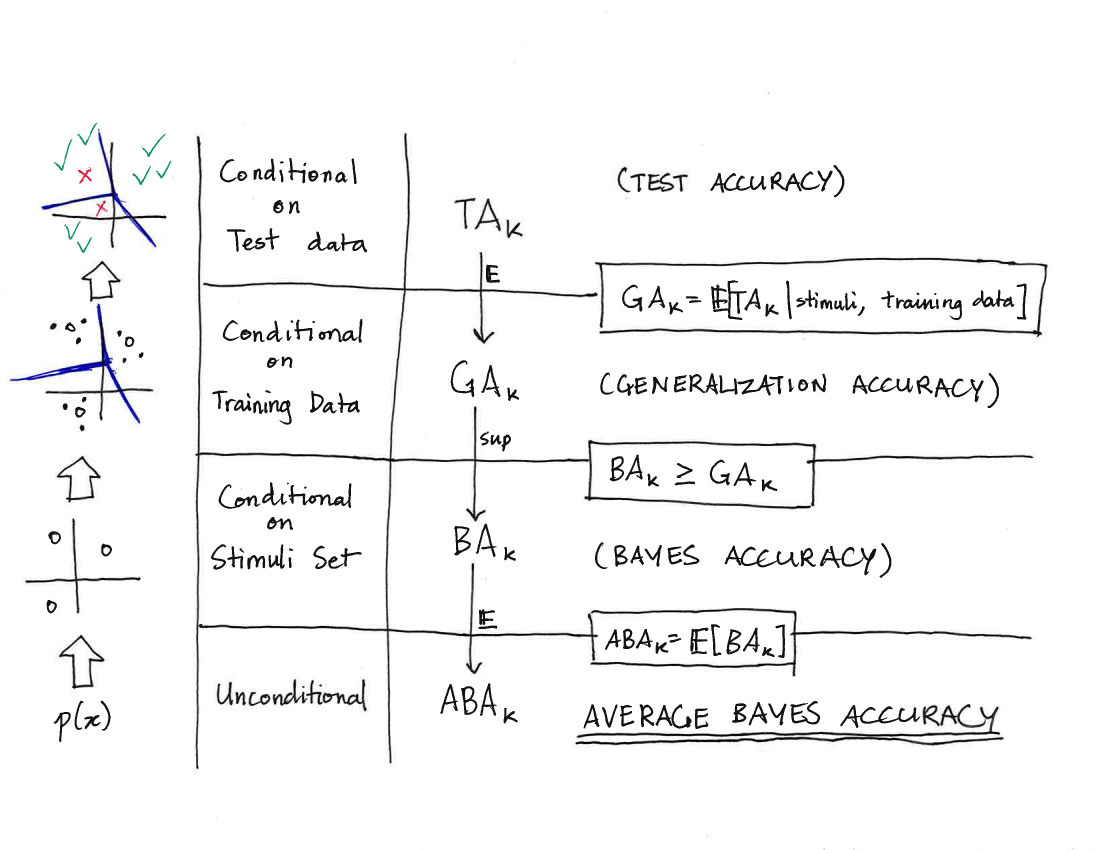
\includegraphics[scale = 0.3, clip = true, trim = 0in 1in 5.5in 1in]{ta_to_aba.png}
\end{center}   
\end{column}
\end{columns}
We already know how to do steps 1 and 2; now we discuss step 3.
\end{frame}

\begin{frame}
\frametitle{Comparison of ABA and I}
Average Bayes accuracy $\text{ABA}_k[p(x, y)]$ and mutual information $\text{I}[p(x, y)]$ are both \emph{functionals} of $p(x, y)$.
\[
\text{ABA}_k[p(x, y)] = \frac{1}{k} \int p_X(x_1)\hdots p_X(x_k) \max_{i=1}^k p(y|x_i)  dx_1\hdots dx_k dy.
\]
\[
\text{I}[p(x, y)] = \int p(x, y) \log \frac{p(x, y)}{p(x)p(y)} dx dy.
\]
\end{frame}

\begin{frame}
\frametitle{Natural questions}
\begin{itemize}
\item Does $\text{ABA}_k$ close to 1 imply $\text{I}$ large?
\item Does $\text{ABA}_k$ close to $1/k$ imply $\text{I}$ close to 0?
\item Does $\text{I}$ large imply $\text{ABA}_k$ close to 1?
\item Does $\text{I}$ close to $0$ imply $\text{ABA}_k$ close to $1/k$?
\end{itemize}
\end{frame}

\begin{frame}
\frametitle{Does $\text{I}$ close to $0$ imply $\text{ABA}_k$ close to $1/k$?}
Answer is yes, since $\text{I}[p(x, y)] = 0$ implies that $X$ is independent of $Y$.
And when $X \perp Y$, the best classifier does not better than random guessing.
\end{frame}

\begin{frame}
\frametitle{Does $\text{I}$ large imply $\text{ABA}_k$ close to 1?}
Answer is \textbf{no}... per the following counterexample.
\begin{columns}
\begin{column}{0.5\textwidth}
\begin{center}
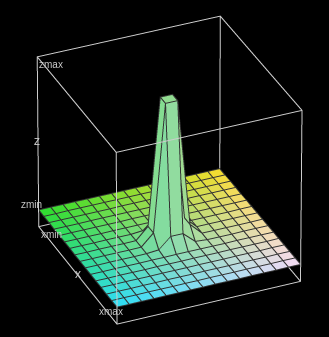
\includegraphics[scale = 0.3]{witch_hat_func.png}
\end{center}
\end{column}
\begin{column}{0.5\textwidth}
\[
X \in [0,1],\ Y \in [0,1]
\]
\[
p(x, y) \propto (1- \alpha) + \alpha \left( \frac{e^{-\frac{x^2 + y^2}{2\sigma^2}}}{2\pi\sigma^2} \right)
\]
\[
\text{I}[p(x, y)] \approx \alpha(\frac{1}{2}\log \frac{1}{\sigma^2} - 1- \log (2\pi))
\]
\end{column}
\end{columns}
Taking $\alpha \to 0$ and $\sigma^2 \leq e^{-\frac{1}{\alpha^2}}$, we get 
\[\text{I}[p(x, y)] \to \infty,\ \ \text{ABA}_k[p(x, y)] \to \frac{1}{k}.\]
This also answers ``\emph{Does $\text{ABA}_k$ close to $1/k$ imply $\text{I}$ close to 0?''} (Also no.)
\end{frame}

\begin{frame}
\frametitle{Natural questions}

\begin{itemize}
\item Does $\text{ABA}_k$ close to $1/k$ imply $\text{I}$ close to 0? \textbf{No}. (counterexample)
\item Does $\text{I}$ large imply $\text{ABA}_k$ close to 1?  \textbf{No}. (counterexample)
\item Does $\text{I}$ close to $0$ imply $\text{ABA}_k$ close to $1/k$? \textbf{Yes}.
\end{itemize}

The only remaining question is:
\vspace{0.2in}

Does $\text{ABA}_k$ close to 1 imply $\text{I}$ large?
\vspace{0.2in}

The answer is yes and provides the desired lower bound.  In fact,
\[
\text{ABA}_k \to 1
\]
implies
\[
\text{I}[p(x, y)] \to \infty.
\]
\end{frame}

\begin{frame}
\frametitle{Problem formulation} Take $\iota > 0$, and fix $k \in
\{2,3,...\}$.  Let $p(x, y)$ be a joint density (where $(X, Y)$
could be random vectors of any dimensionality.)  Supposing
\[
\text{I}[p(x, y)] \leq \iota,
\]
then can we bound
\[
\text{ABA}_k[p(x, y)]?
\]

In other words, does there exist a constant
\[
C_k(\iota) = \sup_{p(x, y): \text{I}[p(x, y)] < \iota} \text{ABA}_k[p(x, y)]?
\]
\end{frame}

\begin{frame}
\frametitle{Step 1: Reduction}
Let $\mathcal{P}^{unif}$ be the class of densities $p(x, y)$ on the unit square, with uniform marginals
\[
p(x) = 1,\ \ p(y) = 1.
\]
We can show that if $C_k(\iota)$ exists, then we need only to search through distributions in $\mathcal{P}^{unif}$ to compute it:
\[
C_k(\iota) = \sup_{p(x, y) \in \mathcal{P}^{unif}: \text{I}[p(x, y)] < \iota} \text{ABA}_k[p(x, y)].
\]
We omit the proof.
\end{frame}

\begin{frame}
\frametitle{Step 1: Reduction}
Reduction simplifies the formulas.  For $p(x, y) \in \mathcal{P}^{unif}$,
\[
\text{I}[p(x, y)] = \int p(x, y) \log p(x, y) dx dy,
\]
and
\[
\text{ABA}_k[p(x, y)] = \frac{1}{k}\int \max_{i=1}^k p(x_i, y) dx_1 \cdots dx_k dy.
\]
\end{frame}

\begin{frame}
\frametitle{Step 2: Conditioning}
Due to uniform marginals $p(x, y) = p(x|y) = p(y|x)$.  Therefore,
\[
\text{I}[p(x, y)] = \int p(x|y) \log p(x|y) dx dy,
\]
and
\[
\text{ABA}_k[p(x, y)] = \frac{1}{k}\int \max_{i=1}^k p(x_i|y) dx_1 \cdots dx_k dy.
\]
\end{frame}

\begin{frame}
\frametitle{Step 2: Conditioning}
Write both functionals as an nested integral, with the outer integration over $y$
\[
\text{I}[p(x, y)] = \int \left[\int p(x|y) \log p(x|y) dx\right] dy,
\]
and
\[
\text{ABA}_k[p(x, y)] =\int \left[\frac{1}{k} \int \max_{i=1}^k p(x_i|y) dx_1 \cdots dx_k\right] dy.
\]
Notice that in both cases, the inner integral is a functional of $p(x|y)$.
\end{frame}

\begin{frame}
\frametitle{Step 2: Conditioning}
Name the functionals, as \emph{conditional information}
\[
\text{I}[p(x, y)] = \int \underbrace{\left[\int p(x|y) \log p(x|y) dx\right]}_{\text{CI}[p(x|y)]} dy,
\]
and \emph{conditional accuracy}
\[
\text{ABA}_k[p(x, y)] = \int \underbrace{\left[\int\frac{1}{k} \max_{i=1}^k p(x_i|y) dx_1 \cdots dx_k\right]}_{\text{CA}_k[p(x|y)]} dy.
\]
\end{frame}


\begin{frame}
\frametitle{Step 2: conditioning}
Conditional information and conditional accuracies are functionals of one-dimensional densities.
\[
\text{CI}[q(x)] = \int q(x) \log q(x) dx,
\]
\[
\text{CA}_k[q(x)] = \frac{1}{k}\int \max_{i=1}^k q(x_i) dx_1 \cdots dx_k.
\]
And, we have
\[
\text{I}[p(x, y)] = \int \text{CI}[p(x|y)]dy = \E[\text{CI}[p(x|Y)]],
\]
and
\[
\text{ABA}_k[p(x, y)] = \int \text{CA}_k[p(x|y)]dy = \E[\text{CA}_k[p(x|Y)]].
\]
for $Y \sim \text{Unif}[0,1]$.
\end{frame}

\begin{frame}
\frametitle{Step 3: convexity}
\begin{itemize}
\item Given $p(x, y) \in \mathcal{P}^{unif}$, define a map $\phi: [0,1] \to \mathbb{R}^2$
by
\[
\phi(y) = (\text{CI}[p(x|y)], \text{CA}_k[p(x|y)]).
\]
We are mapping observations $y$ to their associated conditional information and accuracy.
\item Consider the image of $\phi$:
\[
\text{Im}(\phi) = \{(\text{CI}[p(x|y)], \text{CA}_k[p(x|y)]): y \in [0,1]\}
\]
\item We have $(\text{I}[p(x, y)], \text{ABA}_k[p(x, y)]) = \E[\phi(y)]$.
\item Therefore,
\[
(\text{I}[p(x, y)], \text{ABA}_k[p(x, y)]) \in \mathcal{C}(\text{Im}(\phi)),
\]
the convex hull of the image of $\phi$.
\end{itemize}
\end{frame}

\begin{frame}
\frametitle{Step 3: convexity}
\begin{itemize}
\item Let $\mathcal{P}^1$ denote the set of all densities $q(x)$ on $[0,1]$. Define the set $S$ as
\[
S: \{(\text{CI}[q(x)], \text{CA}_k[q(x)]): q \in \mathcal{P}^1\}
\]
\item Since all conditional densities $p(x|y) \in \mathcal{P}^1$, we have
\[
\text{Im}(\phi) \subset S,
\]
and therefore
\[
\mathcal{C}(\text{Im}(\phi)) \subset \mathcal{C}(S).
\]
\item Therefore,
\[
(\text{I}[p(x, y)], \text{ABA}_k[p(x, y)]) \in \mathcal{C}(S).
\]
\end{itemize}
\end{frame}

\begin{frame}
\frametitle{References}
\begin{itemize}
\item Cover and Thomas.  Elements of information theory.
\item Muirhead.  Aspects of multivariate statistical theory.
\item van der Vaart.  Asymptotic statistics.
\end{itemize}
\end{frame}

\end{document}









